\documentclass[tikz,border=10pt]{standalone}
% Parallelogram ABCD with point E on AD, interior segments BE and CE
% Coordinates: x=(px-307)*0.014235, y=(182-py)*0.014235 (cm)
\begin{document}
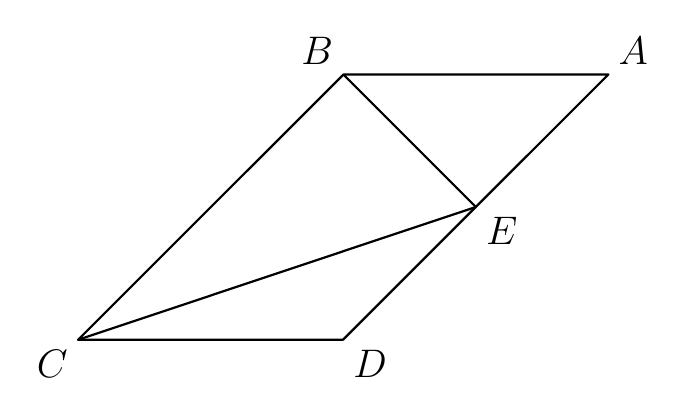
\begin{tikzpicture}[line join=round, line width=0.8pt,
  every node/.style={font=\fontsize{15}{18}\selectfont}]
  % Vertices
  \coordinate (B) at (-0.020939095587845902,1.6765887325367406);
  \coordinate (A) at (3.3440127367721044,1.677704925626948);
  \coordinate (D) at (-0.02706414448169453,-1.6914244906963793);
  \coordinate (C) at (-3.392015976841645,-1.6925406837865868);
  \coordinate (E) at (1.6600064801390804,-0.005328483680722856);

  % Solid edges of the parallelogram
  \draw (B) -- (A) -- (D) -- (C) -- cycle;

  % Interior segments from B and C to E on AD
  \draw (B) -- (E);
  \draw (C) -- (E);

  % Labels
  \node[above left] at (B) {$B$};
  \node[above right] at (A) {$A$};
  \node[below left] at (C) {$C$};
  \node[below right] at (D) {$D$};
  \node[below right] at (E) {$E$};
\end{tikzpicture}
\end{document}
% GEOAGENT_REPAIR_V1 c18a466396f54661 ad1a4978b4fcd11905eec8ac31c5769d05da26cfaa064dd5035f44c02ccc60af
